\documentclass[12pt,a4paper]{article}
\usepackage{enumitem}
% Define margins
\setlength{\topmargin}{-1.0cm}
\setlength{\oddsidemargin}{0.1cm}
\setlength{\textwidth}{16.5cm}
\setlength{\textheight}{23.0cm}

% Use Times New Roman font
\usepackage{times}
\usepackage{xurl}
\usepackage[hidelinks]{hyperref} 
\urlstyle{rm}

\renewcommand{\rmdefault}{ptm}

\usepackage{graphicx} % LaTeX package to import graphics
\graphicspath{{images/}} % Configuring the graphicx package

% Define header and footer
\usepackage{fancyhdr}
\pagestyle{fancy}
\fancyhf{}
\rhead{\textbf{\textit{Week 8 Submission}}}
\cfoot{\textbf{\textit{\thepage}}}
\renewcommand{\headrulewidth}{0.7pt}
\setlength{\headheight}{14pt}

% Adjust section and subsection title formats
\usepackage{titlesec}
\titleformat{\section}
  {\normalfont\fontsize{14}{15}\bfseries}{\thesection}{1em}{}
\titleformat{\subsection}
  {\normalfont\fontsize{12}{15}\bfseries}{\thesubsection}{1em}{}

% Define a style with no footer for the table of contents
\fancypagestyle{nofooter}{%
  \fancyfoot{}%
}

% To manage references
\usepackage{natbib}
\usepackage[labelfont=bf]{caption}

\begin{document}

% TITLE PAGE

\begin{titlepage}

\newcommand{\HRule}{\rule{\linewidth}{0.5mm}}
\center

\vspace*{1\baselineskip}

\includegraphics[width=0.15\textwidth]{images/UTS.png}\\
\textsc{\LARGE University of Technology Sydney}\\[2.0cm]
\textsc{\Large (32557) Enabling Enterprise Information Systems}\\[0.2cm]

\HRule\\[0.6cm]
{\huge\bfseries Acquiring Information Systems and Applications}\\[0.4cm]
\HRule\\[10cm]

\emph{by Team Super} \\
{ Seoyoon Kim (25388442) [Group leader] \\}
{ Jin Lee (25388733)  \\}
{ Ariel Manueke (25207919) \\}
{ Nonthawat Praisompong (25233750) \\}

\vfill
{\large\today}

\vfill

\end{titlepage}

% TABLE OF CONTENTS

\tableofcontents
\thispagestyle{nofooter}
\cleardoublepage

\pagebreak

% DOCUMENT CONTENT STARTS HERE
% You can start writing your document content here.


% Student %%%%%%%%%%%%%%%%%%%%%%%%%%%%%%%%%%%%%%%%%%%%%%%%%%%%%%%%%%%%%%%%%%%%%%%%%%%%%%%%%%%%%%%%%


\setcounter{page}{1}

\section{Question 1}
\subsection{The Importance of Understanding Systems Development in Business}
\label{sec:Question 1}

In today's fast-evolving business landscape, the role of system development cannot be overstated. It's imperative for all members of an organization, irrespective of their department or role, to possess a basic grasp of the systems development process for several compelling reasons \citep{question_1.1}.\\

\noindent \textbf{Enhances Communication and Collaboration}\\
A fundamental understanding of system development enhances communication between departments and IT teams, ensuring that the systems developed meet organizational needs more accurately. It also fosters collaboration, as team members can contribute valuable insights from their respective areas, leading to more comprehensive and effective systems.\\

\noindent \textbf{Drives Innovation and Decision-Making}\\
Knowledge of how systems are developed empowers employees to identify and propose areas for innovation, directly contributing to the organization's competitive edge. It also supports informed decision-making, particularly in technology investments, by providing a clearer understanding of development complexities, potential risks, and realistic timelines.\\

\noindent \textbf{Promotes Responsible System Use}\\
An awareness of the effort and resources involved in system development encourages responsible usage among employees. This responsible use is critical for maintaining system integrity, ensuring security, and providing constructive feedback for continuous improvement.\\

\noindent \textbf{Conclusion}\\
A basic understanding of the systems development process is essential not just for IT professionals but for all organizational members. It underpins effective communication, collaboration, innovation, strategic decision-making, and efficient change management. Moreover, it contributes to the responsible use and continuous improvement of systems, which are crucial for achieving operational excellence and maintaining a competitive edge in the market \citep{question_1.2}.\\



\pagebreak %%%%%%%%%%%%%%%%%%%%%%%%%%%%%%%%%%%%%%%%%%%%%%%%%%%%%%%%%%%%%%%%%%%%%%%%%%%%%%



\setcounter{page}{2}

\section{Question 2}
\subsection{Differences Between Outsourcing, Insourcing, and Offshoring}
\label{sec:Question 2}

\noindent \textbf{Outsourcing vs. Insourcing}\\
Outsourcing refers to the practice where businesses contract out certain tasks or services to external companies or individuals instead of handling them internally. This strategy is often adopted to reduce costs, access specialized skills, or improve focus on core business activities. Outsourcing can involve both domestic and international vendors.\\

\noindent Insourcing, on the other hand, involves bringing tasks or services in-house, where they are managed by the company’s own employees. This approach can offer greater control over the project, foster innovation, and enhance collaboration within the organization. Insourcing might be preferred when confidentiality, quality control, or building internal expertise is a priority \citep{question_2.1}.\\

\noindent \textbf{Outsourcing vs. Offshoring}\\
While outsourcing is about hiring external parties to perform tasks, regardless of their location, offshoring specifically refers to relocating certain business processes or services to another country. Offshoring is often driven by the potential for cost savings due to lower labor costs in the destination country. It's worth noting that offshoring can be a form of outsourcing when a company hires a foreign third-party service provider. However, a company can also offshore tasks without outsourcing, by setting up its own subsidiary or branch in a foreign country to handle these tasks (known as ``captive offshoring'').\\

\subsection{Personal Perspective as a CEO}

If I were the CEO of a large corporation, my decision to outsource, offshore, or insource would heavily depend on the specific circumstances and strategic goals of my company. However, here are some general considerations:

\begin{itemize}
    \item \textbf{Outsourcing:} I would consider outsourcing for non-core activities where external firms have specialized expertise that could significantly benefit my company. This could include IT services, payroll, and customer support. Outsourcing these tasks could allow my company to focus on its core competencies and strategic objectives.
    \item \textbf{Offshoring:} I might consider offshoring if the cost benefits are substantial and if the offshored activities do not compromise the quality of our offerings or the integrity of our operations. This approach would be more appealing for processes that are labor-intensive and standardized, such as manufacturing or basic data entry. However, I would also weigh the potential downsides, such as cultural and language barriers, which could impact service quality and brand reputation.
    \item \textbf{Insourcing:} For activities that are central to our competitive advantage or require tight control and coordination, insourcing would be my preferred option. This includes R\&D, strategic planning, and any other area where maintaining proprietary knowledge and fostering innovation is crucial. Insourcing these functions can promote agility, improve quality control, and ensure that critical knowledge and skills are retained within the company.
\end{itemize}

\noindent Ultimately, the choice among outsourcing, offshoring, and insourcing would be based on a thorough analysis of costs, benefits, risks, and how each option aligns with the company's long-term strategic goals \citep{question_2.2}. Factors such as the need for control, the importance of quality, cost considerations, and the potential for innovation would all play a critical role in this decision-making process.


\pagebreak

% Jin%%%%%%%%%%%%%%%%%%%%%%%%%%%%%%%%%%%%%%%%%%%%%%%%%%%%%%%%%%%%%%%%%%%%%%%%%%%%%%%

\setcounter{page}{4}

\section{Question 3}
\subsection{Three of the most disastrous IT projects around the globe}
\label{sec:Question 3}
\nocite{question_3.1}

\begin{itemize}
    \item Quibi’s Demise
    \item Denver International Airport’s Automated Baggage System
    \item Sainsbury’s warehouse automation
\end{itemize}

\subsection{Reason for Quibi’s failure}
\label{sec:Question 3}
\nocite{question_3.2}

\begin{itemize}
    \item \textbf{Content and Format Considerations in Quibi's Strategy: }Quibi's initiative sought to disrupt the entertainment sector by offering concise, mobile-optimized visual narratives. Yet, the venture faced challenges in curating a portfolio of content that garnered widespread appeal, failing to produce signature programs or viral phenomena essential for subscriber acquisition.
    
   \item \textbf{Market Dynamics and Competitive Landscape: }Upon its foray into the streaming arena, Quibi confronted a saturated marketplace, governed by well-established entities such as Netflix, Amazon Prime, and Hulu. These incumbents provided a diverse array of content, encompassing both short-form and feature-length productions, overshadowing Quibi's offerings and contributing to its competitive disadvantage.
    
   \item \textbf{Assessment of Pricing Structure and Perceived Value: }Despite its focus on mobile accessibility, Quibi's pricing model aligned with those of comprehensive streaming services, complicating its ability to delineate a distinct and persuasive value proposition to its prospective audience.

    \item \textbf{Influence of the COVID-19 Health Crisis on Media Consumption Patterns: }The pandemic's onset and consequent confinement measures precipitated a shift in media consumption behaviors, reducing the demand for mobile-exclusive content. This shift substantially impacted Quibi's foundational value proposition, which emphasized on-demand entertainment for the mobile user.

    \item \textbf{User Interface and Experience Impediments: }Reports from users indicated obstacles interacting with Quibi's application interface and operational aspects. These reported complications potentially inhibited subscriber growth and contributed to increased rates of service discontinuation.

    \end{itemize}
    
\subsection{Concluding Remarks on IT Project Failures}
\label{sec:Question 3}
\nocite{question_3.3}

\noindent IT projects often harbor the potential for groundbreaking advancements, yet they are not immune to failure, as the case of Quibi has demonstrated. Common threads that contribute to the demise of such projects include a misalignment between product offerings and market needs, as seen in Quibi's content format struggles. Additionally, fierce competition within a saturated market can overshadow new entrants, making it challenging to secure a foothold, as evidenced by Quibi's challenge in establishing its niche against streaming behemoths like Netflix, Amazon Prime, and Hulu.

\noindent The pricing strategy and value proposition are also crucial elements; Quibi's parallel pricing with larger, more diverse platforms failed to attract customers seeking value for money. Furthermore, external factors such as societal shifts—in this instance, the COVID-19 pandemic—can rapidly and unpredictably alter consumer behavior, rendering a product's value proposition obsolete. Lastly, technical challenges and user experience issues, if not promptly and adequately addressed, can deter potential users and escalate customer attrition rates.\\

\noindent These factors, collectively, underscore the necessity for thorough market research, adaptive strategy planning, rigorous testing of product functionality, and continuous engagement with user feedback. Successful IT projects typically display a keen understanding of their target market, a clear and compelling value proposition, and the agility to pivot when confronted with unforeseen market dynamics or internal project hurdles.\\

\noindent To mitigate the risk of failure, IT projects should also include a contingency plan, transparent communication with stakeholders, and the inclusion of end-user insights throughout the development process. The lessons learned from Quibi's story, alongside scholarly research on IT project management, provide invaluable insights for practitioners in the field.\\

\noindent The above article referenced the following references:
\begin{itemize}
    \item \cite{Ref3.1}.
    \item \cite{Ref3.2}.  
    \item \cite{Ref3.3}.  
\end{itemize}

\pagebreak

% PAP%%%%%%%%%%%%%%%%%%%%%%%%%%%%%%%%%%%%%%%%%%%%%%%%%%%%%%%%%%%%%%%%%%%%%%%%%%%%%%%

\setcounter{page}{6}
\section{Question 4}
\subsection{Alternative Development Methods Other Than SDLC}
\label{sec:Question 4}

\subsubsection{Kanban}

\begin{quote}
Kanban is a methodology used for work management to maximize development pro-gress and efficiency. It serves as a template for tracking progress and managing task planning. It functions as a progress tracker of a backlog (features to be made) from planning, in progress, testing, or validation, to completion. Each status is grouped and mapped in the same column, easily identified visually by the placement of the backlog. Here is the basic structure template of the Kanban Board:    
\end{quote}

\begin{figure}[htbp]
    \centering
    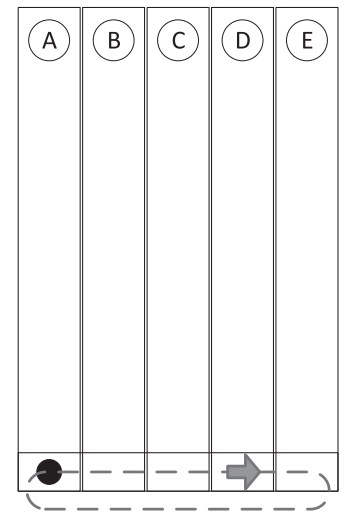
\includegraphics[width=0.3\textwidth]{images/kanban structure.png}
    \caption{Structure Template Kanban Board \citep{question_4.1}}
    \label{fig:example}
\end{figure}

\begin{quote}
    Kanban is a powerful method used to track development work within a team. Multiple Kanban templates are used, with some customization, by various organizations. The simplest implementation involves using a table to map the backlog, to-do, progress, testing, and done. The backlog contains information about the feature/goal to be pursued, estimated completion time, and task priority. The to-do list helps the development team identify and plan actions to start work on a particular backlog. Progress displays all backlogs currently in development. Testing indicates that the backlog has been built and is ready to be tested or validated according to requirements. Finally, all backlogs that pass the quality test are moved to the done column. Here is the Kanban board template:
\end{quote}

\begin{figure}[htbp]
    \centering
    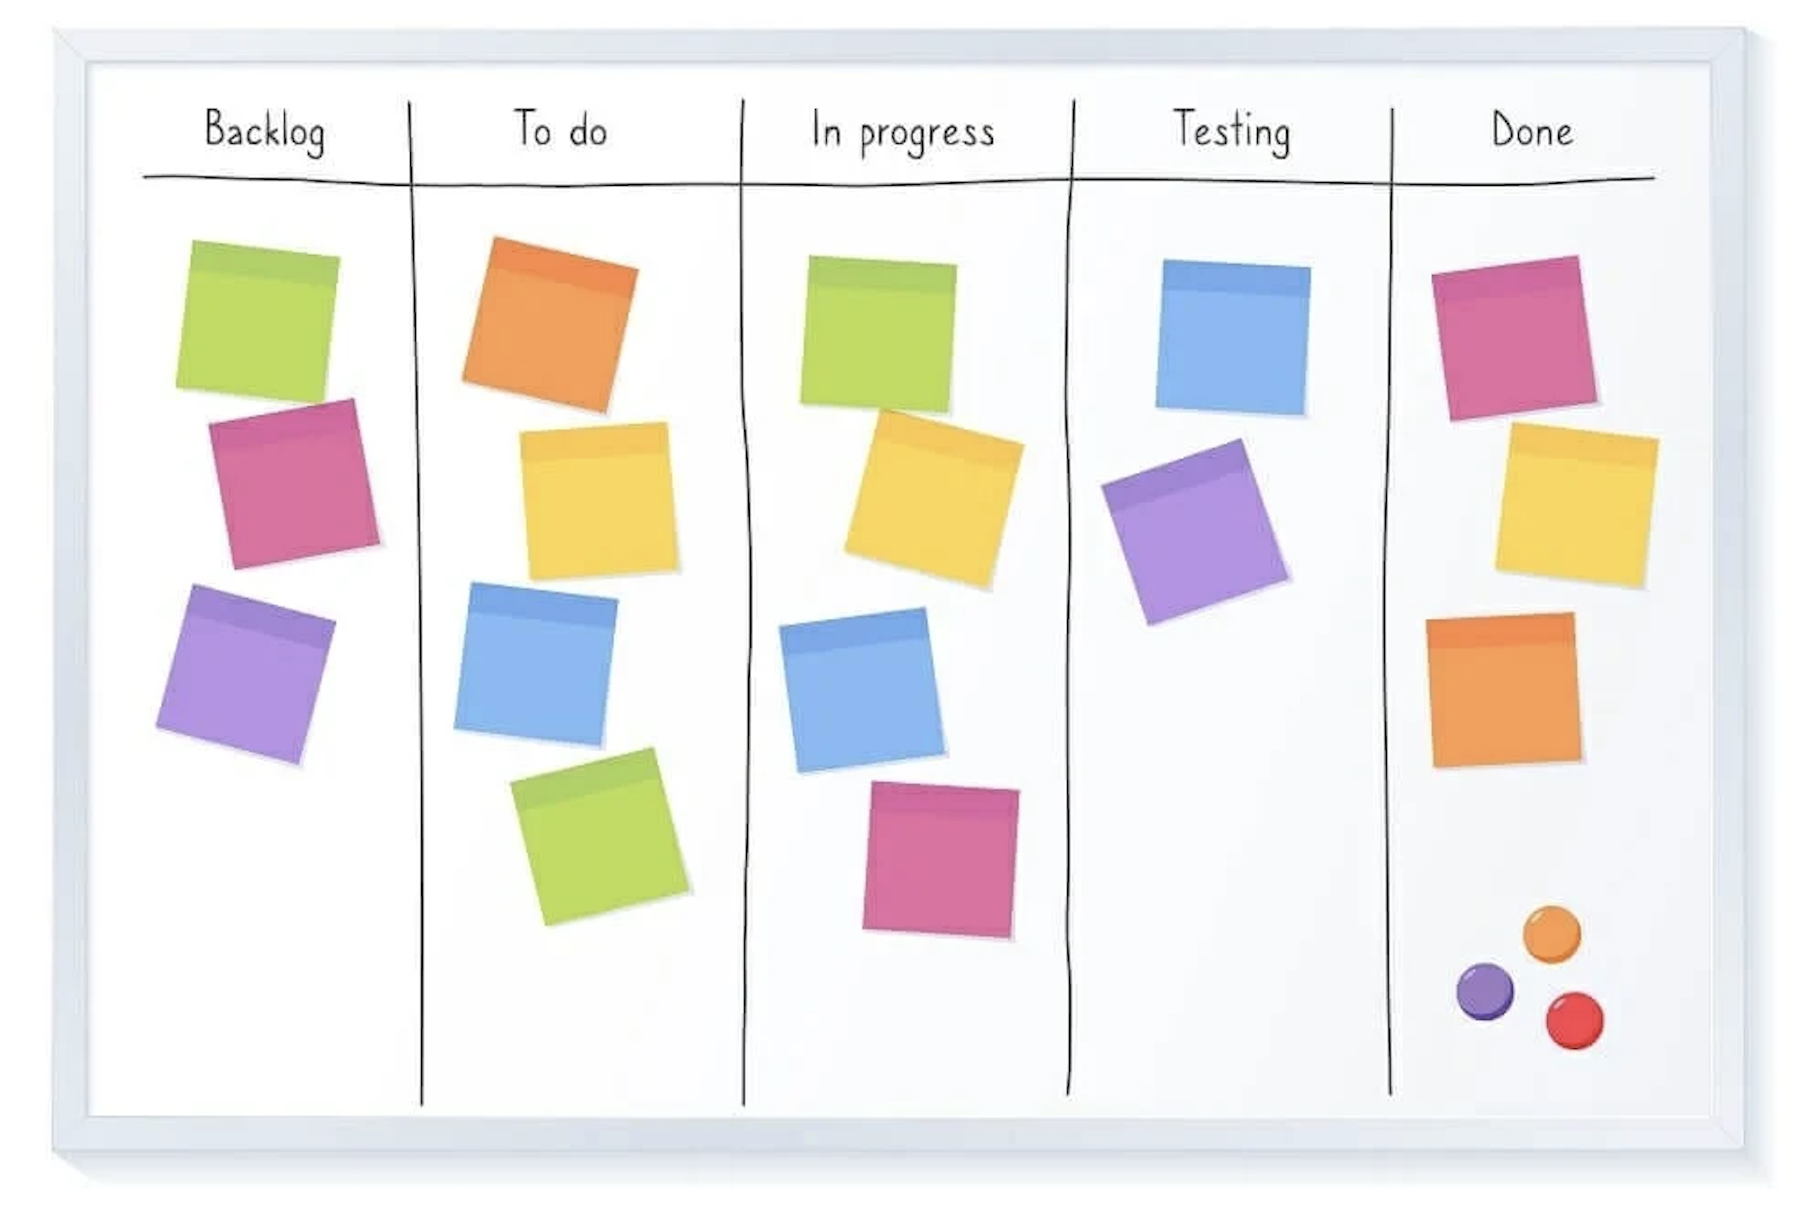
\includegraphics[width=0.7\textwidth]{images/kanban board.png}
    \caption{Kanban board template \citep{question_4.2}}
    \label{fig:example}
\end{figure}

\newpage
\subsubsection{Scrum}

\begin{quote}
Scrum is part of the agile methodology that essentially should have flexibility and is adaptable to changes of need during the development process. The Scrum team consists of the Scrum master, product owner, and developers who need to collaborate effectively because it is one of the most important success factors for the agile methodology success \citep{question_4.3}. Here is the scrum framework introduced by Kenneth S. Rubin:
\end{quote}

\begin{figure}[htbp]
    \centering
    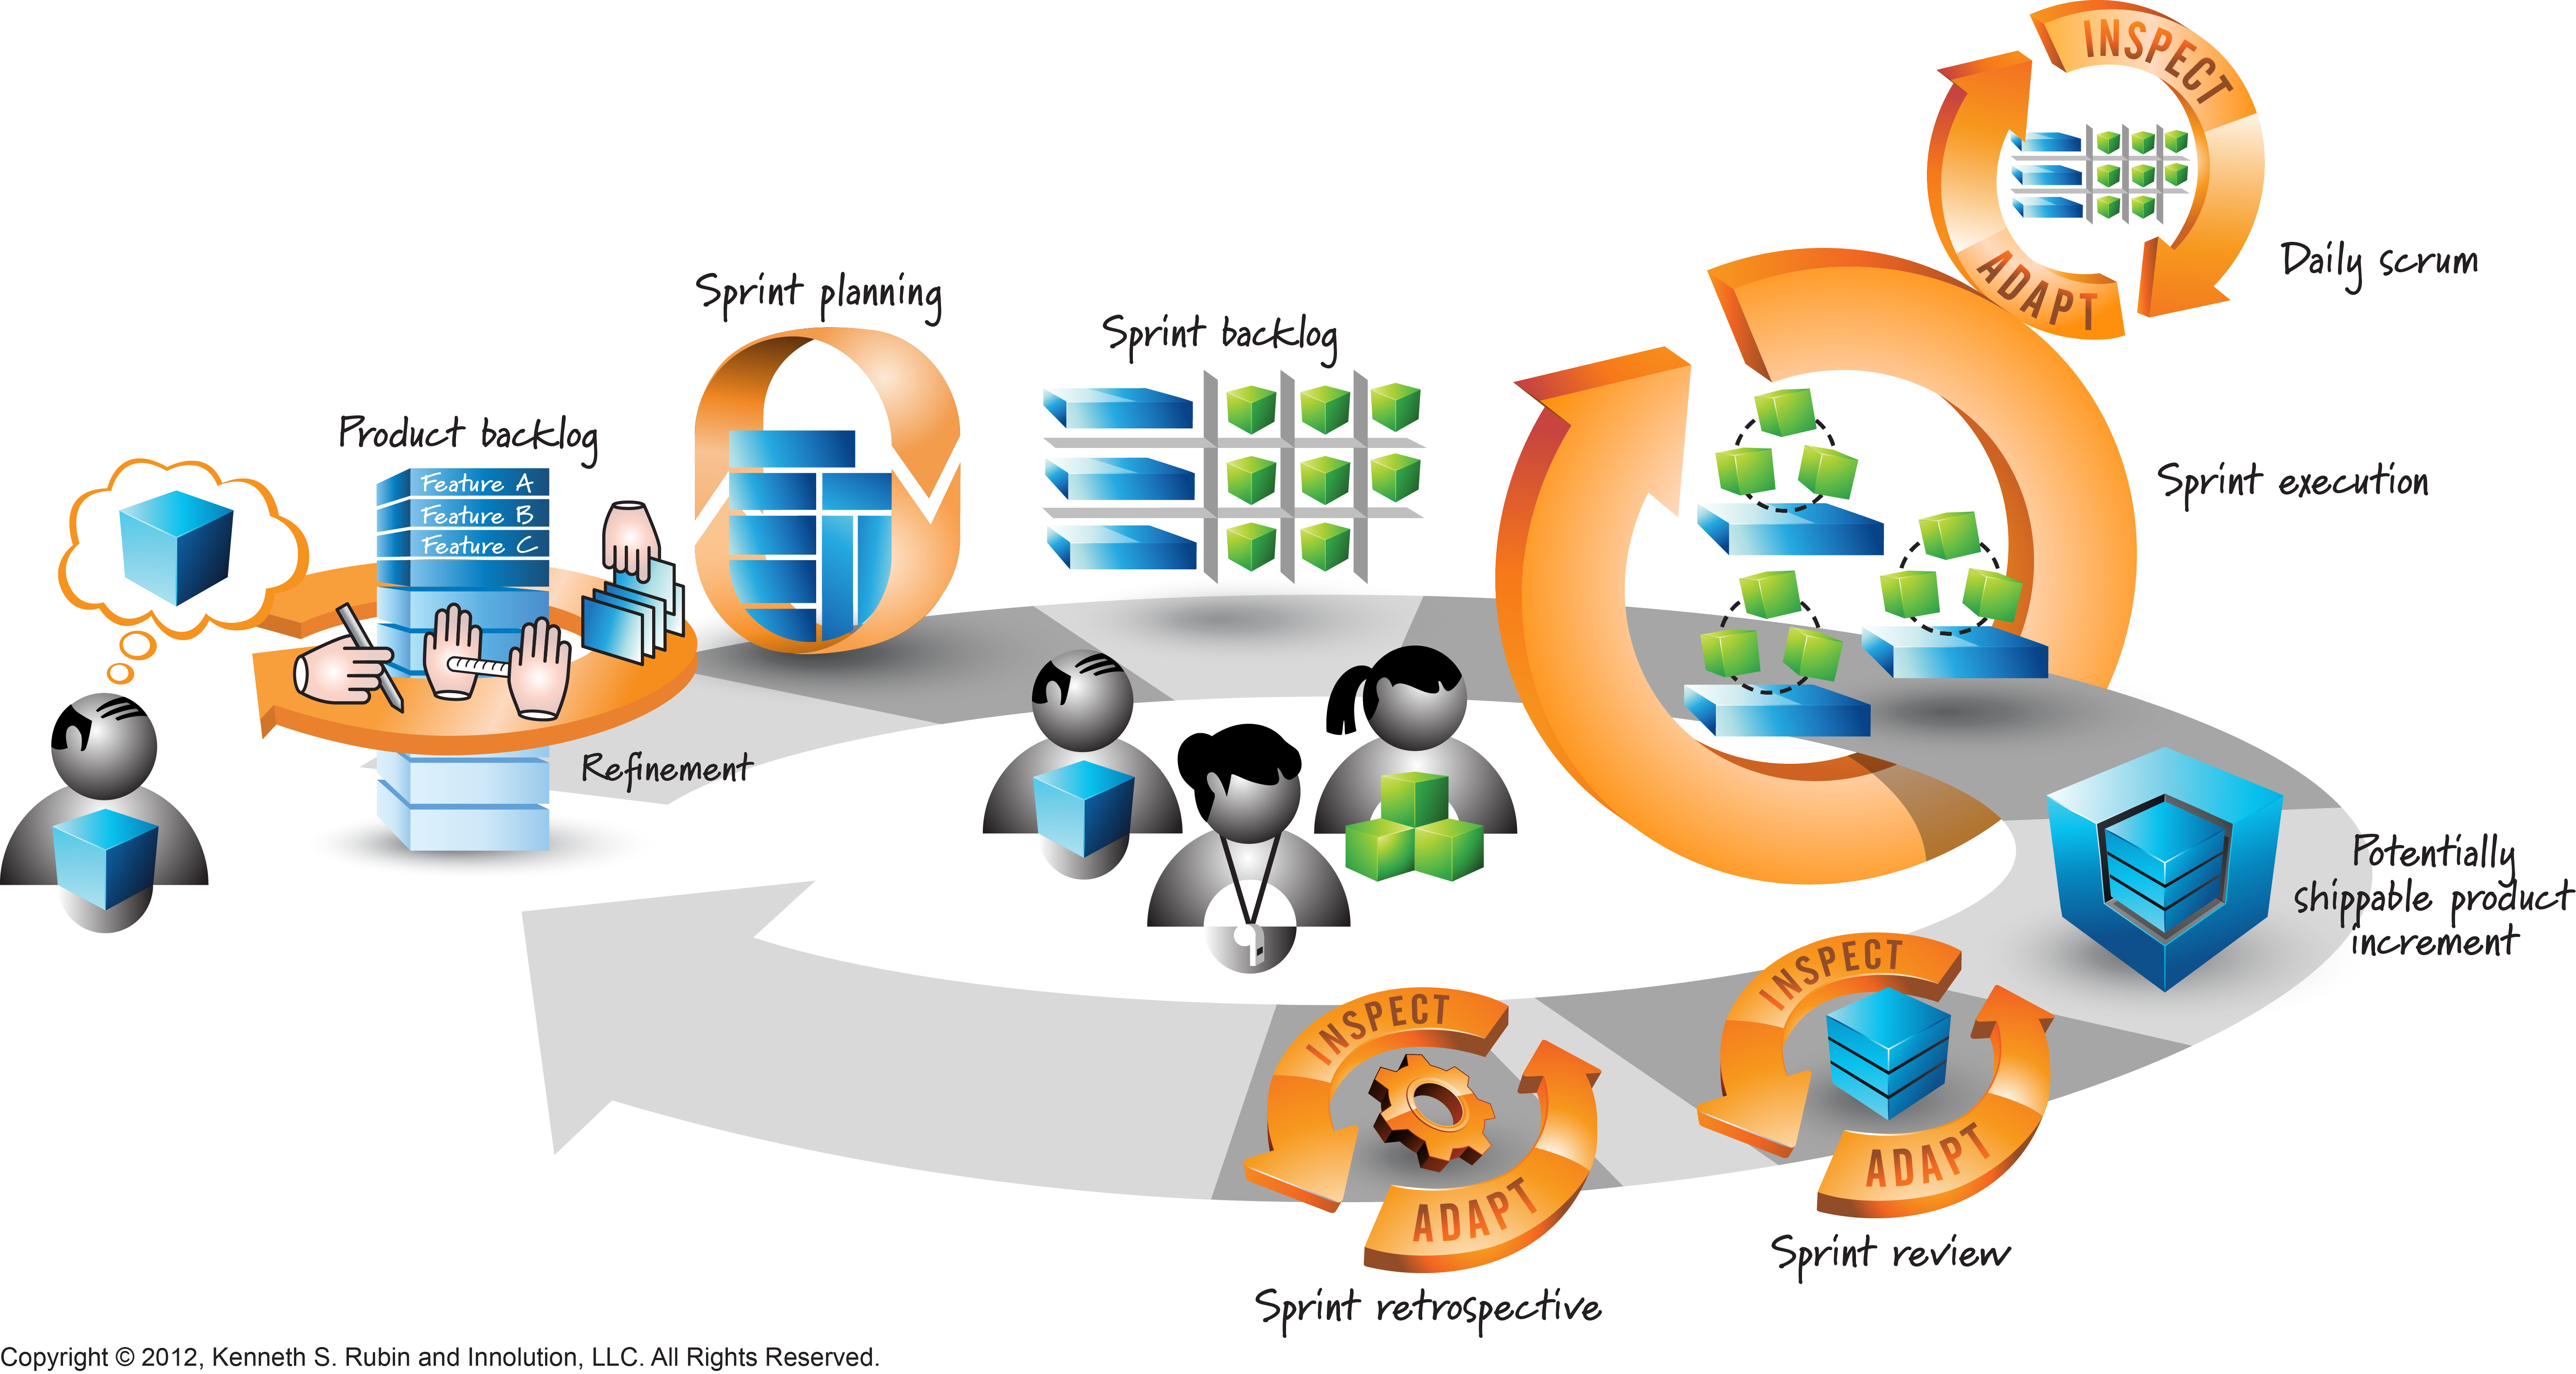
\includegraphics[width=0.7\textwidth]{images/sprint cycle.png}
    \caption{Scrum Sprint Process \citep{question_4.4}}
    \label{fig:example}
\end{figure}

\begin{quote}
According to Figure m, the Scrum framework begins with discussions between the product owner and stakeholders to determine the features to be built, progressing through multiple refinement stages until the product backlog is produced. Following this, the Scrum team (comprising the Scrum master, product owner, and developers) plans the sprint and creates a sprint backlog, serving as a blueprint for the team's execution \citep{question_4.3}. 
\end{quote}

\begin{quote}
During the sprint execution phase in Figure m, developers work on each chosen sprint product backlog to produce a working feature or product in a cycle process known as sprint execution. Throughout this phase, daily scrums, 15-minute meetings facilitated by the Scrum master, occur to update progress, address barriers, and establish action plans for each team member, ensuring the smooth operation of the Scrum process \citep{question_4.3}. 
\end{quote}

\begin{quote}
The outcome of each sprint, according to Figure m, is a potentially shippable product increment, ready to be merged with other finished-executed backlogs, gradually growing from a small-scale to a full-scale system. Subsequently, the team conducts a sprint review to assess results and determine any revisions to be added to the next sprint. Finally, a sprint retrospective is held for the team to reflect on challenges and identify actions to enhance effectiveness in subsequent sprints \citep{question_4.3}. 
\end{quote}

\begin{quote}
This entire process, from determining the product backlog to the sprint retrospective, constitutes one sprint, typically lasting 2 to 4 weeks depending on the product's complexity.
\end{quote}

\subsection{Alternative Development Tools Other Than Prototyping}

\subsubsection{Jira}

\begin{quote}
Jira is a project management tool that helps the software development team to organize, plan, track, and manage the project efficiently. Both methodologies above, Kanban and Scrum also supported by Jira software. Jira can be accessed through the website with a registered account. Once the project is created, the team can start creating the tasks and assign each task to the person in charge. Some information will attached to a task including deadline, comment, supporting document, links, etc. With Jira team can track the progress and status of each task as well as manage the documentation report neatly. Jira also connects and integrates with multiple software such as GitHub, Miro, Figma, Teams, etc., which are also often used by developers.
\end{quote}

\subsubsection{Bootstrap}

\begin{quote}
Bootstrap is another tools that provide the template for building a responsive and fast front end and user interface of a website, instead of coding manually using HTML, CSS, and Java Script. This open-source framework can help to boost development time by just using the predefined template to make the interface that can be customized. Developing a website can also be challenging to accommodate various screen sizes and ratios, that’s why Bootstrap is a good idea as it has a responsive design interface that will match with user’s screen. To use Bootstrap simply just go to its documentation, copy and paste the code, or even modify it, and the user interface is ready to be used visually (needs to be set up logically). 
\end{quote}


\pagebreak
%%%%%%%%%%%%%%%%%%%%%%%%%%%%%%%%%%%%%%%%%%%%%%%%%%%%%%%%%%%%%%%%%%%%%%%%%

\setcounter{page}{9}
\section{Question 5}
\subsection{Choices for entrepreneurs and small business owner’s approach}
\label{sec:Question 5}

\textbf{Leasing Software}\\
Many small businesses and entrepreneurs have limited resources for each part of business activities, directly affecting their investment move. According to \cite{question_5.1}. Every business must invest in the appropriate technology to create a competitive advantage. Furthermore, software leasing is the most suitable option for a company like Entrepreneurs that does not have a huge amount of funding. 

\noindent Businesses can use the software without investing in equipment and time by leasing. However, businesses must pay a monthly fee to extend the software's use period due to the advancement of technology. It affects software outdated easily. Lease agreements participate in this by providing an add-on feature and patch for business \citep{question_5.1}.

\noindent\textbf{Example:} Microsoft 365

\subsection{Choices for Big Company approach.}

\textbf{Software-as-a-service (SaaS)}\\
Software-as-a-service (SaaS) provides high-end software that helps businesses access how the data has been organised, and each software is designed based on organisational objectives with SaaS architecture \citep{question_5.2}. Like leasing software, organisations must pay monthly subscriptions for licences that help them reduce equipment and maintenance costs, and It makes it convenient for the whole organisation to access the software by downloading and accessing the software via the Internet.

\noindent\textbf{Example:} Salesforce\\

\noindent\textbf{Employ Continuous Development}\\
The vendor has provided the software following the businesses' particular purpose, which helps businesses access how the data has been organised. Moreover, this method allows employees within the organisation to develop the software based on the company's purpose. For example, the company has bought the licences for Tableau. According to an agreement, the company can modify the software to satisfy the company itself. This means they can modify almost everything by following the conditions. \\

\noindent\textbf{Conclusion}\\
We live in an era of technology that can create competitive advantages and drawbacks for the whole business. In addition, businesses can choose from many appropriate tools based on their specific purpose to make their convenience. However, they must consider their investment carefully because It can cause negative consequences if they cannot maximise the tools they bought. They inevitably have to invest in IT infrastructure to gain a competitive advantage, which can increase both efficiency and effectiveness.


\pagebreak
% BIBLIOGRAPHY %%%%%%%%%%%%%%%%%%%%%%%%%%%%%%%%%%%%%%%%%%%%%%%%%%%%%%%%%%%%%%%%%%%%%%%%%%%%%%%%%%%% 

% Use Leeds Harvard referencing template
\bibliographystyle{lsharvard}
% Add here the bib file with your references
\bibliography{references}
	
\def\UrlBreaks{\do\/\do-}

\clearpage
\end{document}
